\section{Detailed Experimental Setup}
\label{app:experimental_setup}

\subsection{Infrastructure, Datasets, and Reporting Window}
\label{app:infra_dataset_reporting}

We use veRL~\cite{sheng2025hybridflow} v0.7.0 with vLLM~\cite{kwon2023efficient} v0.11.2.
The training pipeline uses Ray for distributed execution, FSDP for actor training, and vLLM as the rollout backend.
All experiments are conducted on a single node with 8 NVIDIA A100-SXM4-80GB GPUs.
We use the SimpleRL math datasets~\cite{zeng2025simplerl}.
SimpleRL-8k-hard and SimpleRL-8k-medium correspond to MATH~\cite{hendrycks2021measuring} Level 3--5 and Level 1--4 problems, respectively.
Following the SimpleRL recipe, we use SimpleRL-8k-hard for the Qwen models and easier one for Llama3.1-8B-Instruct, reflecting the stronger reasoning capability of the Qwen base models in this setting~\cite{zeng2025simplerl}.
For timing summaries, we exclude the first training step because it includes one-time distributed setup and CUDA-graph initialization overheads that do not repeat in steady-state training.
All reported averages are computed over the following 100 steps.


\subsection{Metric Measurement Details}
\label{app:metric_measurement}

For all methods, preparation time, rollout-generation time, and step time are measured throughout training and averaged over training steps.
For \methodtitle{}, the draft length can change only at step boundaries; we therefore report $\mal$ and $\bar{\gamma}$ averaged over training steps, so $\bar{\gamma}$ need not be an integer.
We compute $\alpha$ from the measured $\mal$ using the equation $\mal=(1-\alpha^{\DraftLength+1})/(1-\alpha)$.
When $\gamma$ varies over training, we apply the same inversion within fixed-$\gamma$ portions of the trajectory and average the resulting rates weighted by the number of training steps in each portion.
Preparation time includes method-specific overhead required to enable SD.
For \history{}, it includes rollout-history caching and loading overhead; prefix-matching costs incurred during generation are included in Rollout Gen.
For \Learned{}, it includes hidden-state extraction, which incurs negligible overhead in our implementation, and online drafter-training overhead, including drafter forward/backward passes and optimizer updates.
For \alwayssd{} and \methodtitle{}, it includes per-step drafter quantization overhead.


\subsection{Training and Method Configuration}
\label{app:training_method_config}

We use a train batch size of 128 and generate 8 rollouts per prompt, with a maximum rollout length of 8,192 tokens.
Training is performed with a learning rate of $5\times 10^{-7}$ and a mini-batch size of 128.
Because each mini-batch contains samples from the current policy only, training is purely on-policy and does not require policy-ratio clipping.
The default sampling temperature is set to 1.0 with data parallelism (TP=1).
For the Qwen base models, we use a KL loss coefficient of $10^{-4}$ following SimpleRL~\citep{zeng2025simplerl}, and for the Llama instruct model, we use $10^{-2}$ following FastGRPO~\citep{zhang2025fastgrpo}.
For training stability, we further apply token-level rejection sampling [0.5, 2.0] and frequency penalty 0.05 for Qwen2.5-14B.
For \adaptivepolicy{}, we use the same configuration for all models: $\Gamma=\{5,7,9,11\}$, $\alpha_{\mathrm{up}}=0.94$, $\alpha_{\mathrm{down}}=0.85$, and $P=2$.
We omit $\gamma=3$ because it is consistently dominated by, or comparable to, $\gamma=5$ in the rollout regimes encountered during training.


\subsection{Rollout-History-Based Drafting Baseline}
\label{app:history_drafting}

We use Spec-RL~\cite{liu2025spec} as a representative rollout-history-based drafting baseline.
To our knowledge, it is the only publicly available baseline in this category implemented in a veRL+vLLM training stack.
Spec-RL collects generations from previous epochs and, starting from the second epoch, reuses matching prefixes from this rollout history as draft tokens for the current policy.

This design is not strictly target-distribution preserving.
First, after a token is rejected, Spec-RL does not perform rejection sampling from the corrected target distribution.
Exact SD requires resampling from an adjusted distribution at the first rejected position~\cite{leviathan2023fast}, which in turn requires access to the full probability distribution at that position.
In contrast, rollout-history-based drafting makes exact rejection sampling difficult because it stores only past tokens and their corresponding token probabilities, rather than full logits over the vocabulary for every generated position.
Storing full logits for all positions across an epoch would introduce prohibitive memory and storage overhead.
Second, Spec-RL uses a lenience factor of $e^{0.5}$ in its best-performing configuration to increase the length of reused prefixes.
This heuristic makes token acceptance more permissive, but further departs from exact target-distribution-preserving speculative decoding.
We therefore treat Spec-RL as a lossy rollout-history-based baseline.

\begin{figure}[t]
    \centering

    \begin{subfigure}[t]{0.32\linewidth}
        \centering
        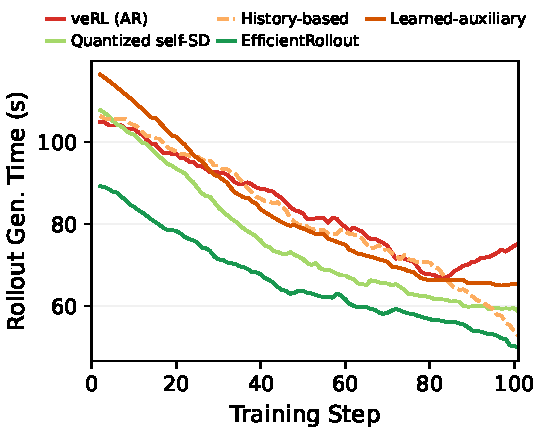
\includegraphics[width=\linewidth]{figures/appendix_gen_time_qwen7b.pdf}
        \caption{Qwen2.5-7B}
        \label{fig:app_qwen7b_gen_time}
    \end{subfigure}
    \hfill
    \begin{subfigure}[t]{0.32\linewidth}
        \centering
        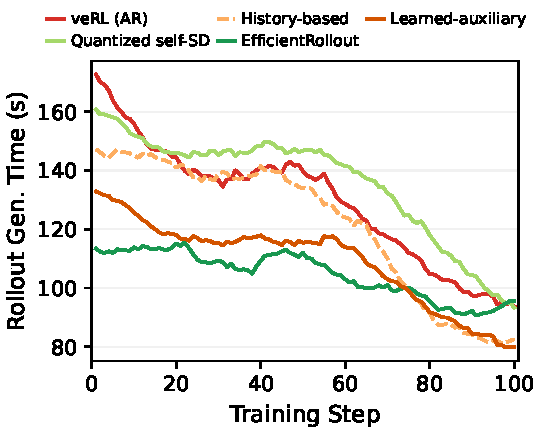
\includegraphics[width=\linewidth]{figures/appendix_gen_time_qwen14b.pdf}
        \caption{Qwen2.5-14B}
        \label{fig:app_qwen14b_gen_time}
    \end{subfigure}
    \hfill
    \begin{subfigure}[t]{0.32\linewidth}
        \centering
        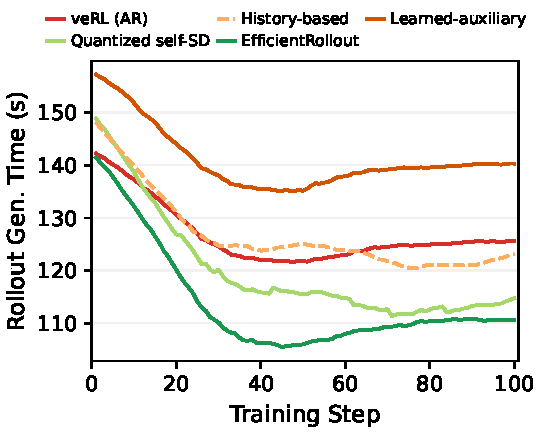
\includegraphics[width=\linewidth]{figures/appendix_gen_time_llama8b.pdf}
        \caption{Llama3.1-8B}
        \label{fig:app_llama8b_gen_time}
    \end{subfigure}

    \caption{
    Rollout-generation time over training steps (smoothed).
    \methodtitle{} consistently reduces rollout time, whereas other SD baselines provide limited gains or can be slower than \nosd{}.
    }
    \label{fig:app_gen_time_breakdown}
\end{figure}


\subsection{Learned Auxiliary Drafting Baseline}
\label{app:learned_auxiliary_drafting}

Existing RL rollout acceleration systems with \learned{} use different execution stacks.
FastGRPO~\citep{zhang2025fastgrpo} uses a HuggingFace Transformers-based rollout pipeline rather than a serving backend such as vLLM or SGLang.
FastRL~\citep{hu2026taming} uses SGLang~\citep{zheng2024sglang} for rollout generation, while NeMo RL~\citep{iso2026accelerating} uses vLLM with NVIDIA's own post-training framework.
A direct system-level comparison would therefore mix drafter design with backend and framework differences, including batching, KV-cache management, SD execution paths, and training-loop implementation.

To isolate the drafter design, we implement an EAGLE3-style \learned{} baseline in the same veRL+vLLM stack used by the other methods in our paper.
A practical requirement of this baseline is that a compatible drafter must be available for each target model family before RL post-training begins.
For Qwen2.5-7B and Qwen2.5-14B, we did not find publicly available compatible EAGLE3 drafters, so we pretrain the drafters on ShareGPT~\citep{aeala2023sharegpt} using the official vLLM SD training pipeline following EAGLE3~\citep{li2025eagle}.
Each drafter is trained for 10 epochs, and we select the checkpoint with the best validation performance.
For Llama3.1-8B-Instruct, we use the publicly available RedHatAI pretrained EAGLE3 drafter~\citep{redhatai2025llama31eagle3}.

For online adaptation during RL, we carefully follow the rollout-SD design choices of FastRL~\citep{hu2026taming} and NeMo RL~\citep{iso2026accelerating}.
Specifically, we capture hidden states during the actor forward pass in the log-probability computation phase and train the drafter inline immediately after each micro-batch of the actor forward.
This avoids cross-step buffering and CPU offload while allowing the drafter to consume the freshly captured target hidden states.
We follow FastRL's packed layout, next-position shift convention, and combined loss with a hidden-regression term and a soft cross-entropy probability-matching term at the 1:0.1 weight ratio; the drafter is trained with a small fixed AdamW learning rate (1e-6).
As a loss-design check, removing the hidden-regression term while keeping only the soft cross-entropy term (matching the NeMo RL formulation) produced similar online block-efficiency trajectories, so we use the FastRL-style combined loss for the primary baseline.
We use a separate AdamW optimizer for the drafter and report the direct drafter-update wall time as method-specific preparation time.

We do not implement FastRL's asynchronous background drafter training, CPU offload, or overlap optimizations.
These techniques introduce additional system-level design choices beyond the drafter itself and would make the comparison depend on overlap efficiency rather than only rollout-time SD behavior.
For decoding, we use chain drafting with a fixed draft length $\gamma=3$, following the best-performing setting reported by~\citet{iso2026accelerating}.
